\documentclass[11pt,a4paper]{article}

\usepackage[T1]{fontenc}
\usepackage[utf8]{inputenc}
\usepackage{lmodern}
\usepackage[margin=1in]{geometry}
\usepackage{amsmath,amssymb}
\usepackage{graphicx}
\usepackage{booktabs}
\usepackage{enumitem}
\usepackage{float}
\usepackage[font=small,labelfont=bf]{caption}
\usepackage[colorlinks=true,linkcolor=blue,citecolor=blue,urlcolor=blue]{hyperref}

% ---------------------------------------------------------------------------
% FILL THESE IN BEFORE SUBMITTING
% ---------------------------------------------------------------------------
% Plain text only here, no angle brackets, so the title page always typesets.
\newcommand{\studentname}{Kshitiz Kumar}
\newcommand{\studentid}{Roll number to be filled}
\newcommand{\studentprogram}{Programme and home institute to be filled}
\newcommand{\internperiod}{Internship dates to be filled}
\newcommand{\drivelink}{https://drive.google.com/drive/folders/REPLACE-WITH-YOUR-FOLDER-ID}
% ---------------------------------------------------------------------------

\setlist{itemsep=2pt,topsep=4pt}
\graphicspath{{../}}

\begin{document}

% ===========================================================================
\begin{titlepage}
\centering
\vspace*{0.6cm}

{\large\scshape Indian Institute of Technology Jodhpur}\\[0.4cm]
{\large Department of Electrical Engineering and Computer Science}\\[0.3cm]
{\large Distributed Systems and Control Laboratory (DSCL)}\\[2.2cm]

{\Large\bfseries Internship Report}\\[1.2cm]

\rule{\textwidth}{0.8pt}\\[0.5cm]
{\LARGE\bfseries Multi-Robot Source Localization and\\[0.3cm]
Formation Control}\\[0.5cm]
{\large Reproducing a Distributed Sign Gradient-Free Algorithm\\
and Extending It to Three Open Problems}\\[0.4cm]
\rule{\textwidth}{0.8pt}\\[2.2cm]

\begin{tabular}{rl}
\textbf{Submitted by} & \studentname\\
                      & \studentid\\
                      & \studentprogram\\[0.6cm]
\textbf{Supervisor}   & Prof.\ Anoop Jain\\
                      & Department of Electrical Engineering\\
                      & and Computer Science\\
                      & IIT Jodhpur\\[0.6cm]
\textbf{Laboratory}   & Distributed Systems and Control\\
                      & Laboratory (DSCL)\\[0.6cm]
\textbf{Period}       & \internperiod\\
\end{tabular}

\vfill
\end{titlepage}

% ===========================================================================
\section*{Acknowledgement}
\addcontentsline{toc}{section}{Acknowledgement}

I am grateful to Prof.\ Anoop Jain for supervising this internship at the Distributed Systems and
Control Laboratory (DSCL), Department of Electrical Engineering and Computer Science, IIT Jodhpur.
The freedom to first rebuild a published result from scratch, and only then to look for what the
result does not cover, shaped the way I now approach a research paper. I also thank the members of
DSCL for their questions during discussions, which repeatedly sent me back to check assumptions I
had taken for granted.

% ===========================================================================
\section*{Abstract}
\addcontentsline{toc}{section}{Abstract}

A group of robots is asked to find the strongest point of an invisible signal, such as a chemical
leak or a heat source, and at the same time hold a circular formation around it. A 2024 paper by
Du and co-authors solves this with a control law that never computes a gradient and lets robots
exchange only the sign of a difference, that is one of the three values $-1$, $0$ or $+1$. Such a
message is very cheap to send, which matters for a real radio link.

This internship did two things. First, the paper was rebuilt from scratch as a working simulator,
in Python and then in MATLAB, for three robot models of increasing realism: ideal point robots,
unicycle robots, and a differential-drive TurtleBot. All three reach the accuracy the paper's
theorem promises. Second, three problems that the paper does not address were identified, worked
out mathematically, and tested in simulation:

\begin{enumerate}[label=(\arabic*)]
    \item \textbf{Many sources.} If the field has $N$ separate sources, the robots must split into
    $N$ teams and each team must surround its own source.
    \item \textbf{A moving source.} If the source keeps moving, the robots can no longer settle on
    it and instead trail behind it.
    \item \textbf{Many peaks.} If the field has several peaks, the robots may lock onto a small one
    and never find the biggest one.
\end{enumerate}

For each problem the report gives the reasoning in plain language, states what was proved, and
reports what the simulation measured. A separate suite of fourteen numerical checks was written to
test each mathematical claim against a measurement instead of trusting the algebra. All fourteen
pass. Two of the checks led to new results that were not in the original plan: one showed that a
condition usually attached to the paper's error formula is never actually needed, and the other
produced an exact formula for an error term that had previously only been known to exist.

\clearpage
\tableofcontents
\clearpage

% ===========================================================================
\section{Introduction}

\subsection{The problem in everyday terms}

Imagine a gas leak inside a large warehouse. The gas concentration is high near the leak and falls
off as you move away. You have a handful of small robots, each carrying a cheap sensor that reports
a single number: how strong the smell is right here. No robot has a map, no robot knows where the
leak is, and no robot can measure which \emph{direction} the smell is getting stronger. Each robot
only gets one number at its own position.

Two things are wanted:

\begin{itemize}
    \item \textbf{Localization.} The robots as a group should end up centred on the leak.
    \item \textbf{Formation.} They should arrange themselves in a ring around it, evenly spaced, so
    that they surround the leak rather than pile up on one side.
\end{itemize}

The quantity being sensed, one number at every point in space, is called a \emph{scalar field}. The
task of driving robots towards its strongest point is called \emph{source seeking}.

\subsection{Why this is harder than it sounds}

The obvious approach is to estimate the direction in which the signal grows, the gradient, and walk
that way. Three practical problems get in the way.

\begin{itemize}
    \item \textbf{One sensor gives no direction.} A single reading is just a number. To get a
    direction, a robot would have to move around and compare readings, which is slow.
    \item \textbf{Noise ruins derivatives.} Real sensors are noisy. Estimating a gradient means
    taking differences of noisy numbers, and differences amplify noise badly.
    \item \textbf{Radio is expensive.} If every robot must broadcast its exact position as a
    floating-point number many times per second, the network becomes the bottleneck long before the
    robots do.
\end{itemize}

The paper this internship started from \cite{du2024} avoids all three. No robot ever estimates a
gradient. Instead, the \emph{ring as a whole} acts as the sensor: the robots sit at known positions
on a circle, and combining their readings with the geometry of the circle recovers exactly the
information a gradient would have given. And robots exchange only signs, so a message is one of
three values per axis rather than a full number.

\subsection{What this internship did}

The work fell into two halves.

\textbf{Half one, reproduction.} The paper was rebuilt from nothing into a working simulator, and
checked against its own theorems rather than against its pictures. Three robot models were built,
each one closer to a real machine than the last.

\textbf{Half two, extension.} Three situations the paper does not cover were identified. For each
one, the mathematics was worked out from the paper's own building blocks, written up properly, and
then tested numerically. A dedicated verification suite was written so that every mathematical
claim has a plot behind it.

Table~\ref{tab:deliverables} lists what exists at the end.

\begin{table}[H]
\centering
\caption{What was produced during the internship.}
\label{tab:deliverables}
\small
\begin{tabular}{@{}p{0.31\linewidth}p{0.62\linewidth}@{}}
\toprule
Item & What it is \\
\midrule
Python simulator & Reference implementation of the paper's control law, with theorem checks,
plots, parameter sweeps and a test suite. \\
MATLAB version & The same model in MATLAB, reading the same configuration files, so results can be
compared across two independent implementations. \\
Three robot models & Point robots, unicycle robots, and differential-drive TurtleBot, as
self-contained MATLAB scripts. \\
Gap simulations & One MATLAB script covering all three new problems, with plots and animations. \\
Verification suite & Fourteen numerical checks, one per mathematical claim. \\
Theory write-ups & Two LaTeX documents: a full research note and a proofs-only companion with every
algebraic step written out. \\
\bottomrule
\end{tabular}
\end{table}

% ===========================================================================
\section{Background: the algorithm we started from}

\subsection{The setting}

There are $n$ robots. Robot $i$ sits at position $p_i$ in the plane. The field being sensed is
strongest at the source $p_s$ and weakens with distance in a simple bowl shape:
\begin{equation}\label{eq:field}
    f(p) = \kappa \, \| p - p_s \|^2 .
\end{equation}
In words: the reading is proportional to the \emph{square} of the distance to the source, and
$\kappa$ says how sharply the field changes. A robot's actual measurement is this value plus a small
amount of noise, and the sensor saturates beyond a maximum range.

Each robot is assigned a fixed slot on a circle of radius $R$. Slot $i$ points in the direction
\begin{equation}\label{eq:slots}
    \phi_i = \left( \cos\theta_i,\ \sin\theta_i \right),
    \qquad \theta_i = \frac{2\pi(i-1)}{n},
\end{equation}
so the slots are spread evenly around the circle. The group's position as a whole is described by
its centroid $p^*$, the average of all the robot positions.

\subsection{The control law, in words}

Every robot adds together two velocity commands.

\textbf{Term one: get into formation.} Robot $i$ compares itself with its neighbours and moves to
reduce the disagreement. The important detail is that it does not use the size of the disagreement,
only its \emph{sign} on each axis. So the message a robot sends is one of $\{-1, 0, +1\}$ per axis.
This is the ``sign'' in sign gradient-free. Using signs also makes this term converge in
\emph{finite} time rather than gradually, which matters because the second term only behaves
correctly once the formation is exact.

\textbf{Term two: move towards the source.} Robot $i$ takes its own scalar reading and moves along
its own slot direction, scaled by that reading. A robot on the far side from the source reads a big
number and pushes hard; a robot on the near side reads a small number and pushes gently. Summed over
the whole ring, the pushes cancel except for a leftover that points at the source. No single robot
knows the direction, but the ring collectively does.

Written out, the command for robot $i$ is
\begin{equation}\label{eq:controller}
    u_i \;=\;
    \underbrace{\alpha \sum_{j \in \mathcal{N}_i} \operatorname{sgn}(z_j - z_i)}_{\text{formation, sign messages only}}
    \;-\;
    \underbrace{\frac{2\beta}{R}\, \sigma_i \, \phi_i}_{\text{move towards the source}},
\end{equation}
where $\sigma_i$ is the reading, $\mathcal{N}_i$ is the neighbour set, $z_i = p_i - R\phi_i$ is a
shifted coordinate that is the same for all robots once the ring is perfect, and $\alpha, \beta$ are
gains the designer picks.

\subsection{Why the ring recovers the gradient exactly}

This is the one piece of algebra worth showing, because everything later depends on it. Because the
slots are evenly spaced, they satisfy two identities:
\begin{equation}\label{eq:moments}
    \sum_{i=1}^{n} \phi_i = 0,
    \qquad\qquad
    \sum_{i=1}^{n} \phi_i \phi_i^{\top} = \frac{n}{2} I_2 .
\end{equation}
The first says the slot directions cancel out. The second says they are spread out evenly in both
axes. Substituting the bowl-shaped field \eqref{eq:field} into the sum of readings weighted by slot
directions, the first identity deletes every term that is the same for all robots, and the second
converts the remaining term into exactly the direction from the group to the source. Nothing is
approximated away. This is why the method works without a gradient estimate, and it is also why the
formation has to be exact before the localization step can be trusted.

\subsection{The two guarantees}

The paper proves two things, and both were used as acceptance tests for the reproduction.

\begin{itemize}
    \item \textbf{Formation in finite time.} If the gain ratio is large enough,
    $\alpha/\beta > 4 n f_{D_{\max}} / R$, then the ring becomes exact after a finite time, not just
    asymptotically.
    \item \textbf{Localization to a known accuracy.} After the ring is exact, the distance from the
    centroid to the source settles inside a radius $\varepsilon$. When every robot can sense the
    source, this simplifies to a very clean formula:
    \begin{equation}\label{eq:epsilon}
        \varepsilon = \frac{\delta}{\kappa R},
    \end{equation}
    where $\delta$ is the noise bound. Read plainly: a bigger ring and a sharper field give better
    accuracy, and more noise gives worse accuracy.
\end{itemize}

% ===========================================================================
\section{How the software is organised}

Everything was built twice on purpose. A bug that appears in one language and not the other is
almost certainly a coding bug; a result that appears in both is much more likely to be real.
Table~\ref{tab:code} lists the pieces used in this report.

\begin{table}[H]
\centering
\caption{Main components of the codebase.}
\label{tab:code}
\small
\begin{tabular}{@{}p{0.26\linewidth}p{0.18\linewidth}p{0.48\linewidth}@{}}
\toprule
Component & Language & Role \\
\midrule
\texttt{sgf\_sim/} & Python & Reference simulator: control law, theorem checks, plots, parameter
sweeps, command-line interface. \\
\texttt{tests/} & Python & Automated tests for the simulator. \\
\texttt{matlab/} & MATLAB & Same model in MATLAB, reading the same JSON configuration files. \\
\texttt{configs/} & JSON & Shared parameter files, so both implementations run identical
experiments. \\
\texttt{sims/SingleIntegrator.m} & MATLAB & Point-robot model, self-contained. \\
\texttt{sims/Unicycle.m} & MATLAB & Unicycle model with feedback linearization. \\
\texttt{sims/TurtleBot.m} & MATLAB & Differential-drive model with wheel speeds. \\
\texttt{sims/research.m} & MATLAB & The three new problems, all in one script. \\
\texttt{sims/verify\_theory.m} & MATLAB & Fourteen checks, one per mathematical claim. \\
\bottomrule
\end{tabular}
\end{table}

Every run writes the same set of files: a trajectory picture, error-versus-time plots, an animated
GIF, a \texttt{summary.json} with all the numbers, and a \texttt{result.mat} with the raw data. Keeping
the output shape identical across every model meant that comparing two runs never required writing
new plotting code. All animations referenced in this report are collected at the shared link given
in \cite{animations}.

% ===========================================================================
\section{Part one: reproducing the paper}

\subsection{Point robots}

The first model treats each robot as a dot that moves exactly where it is told: velocity in,
position out. This is the cleanest possible test of the control law, because nothing about the
robot's body can be blamed for a bad result.

The run uses $n = 6$ robots, a source at $(5.5, 5.5)$, ring radius $R = 2$, noise bound
$\delta = 0.2$, and gains $\alpha = 100$, $\beta = 0.05$. The predicted accuracy from
\eqref{eq:epsilon} is $\varepsilon = 0.2 / (1 \times 2) = 0.1$.

\begin{figure}[H]
\centering
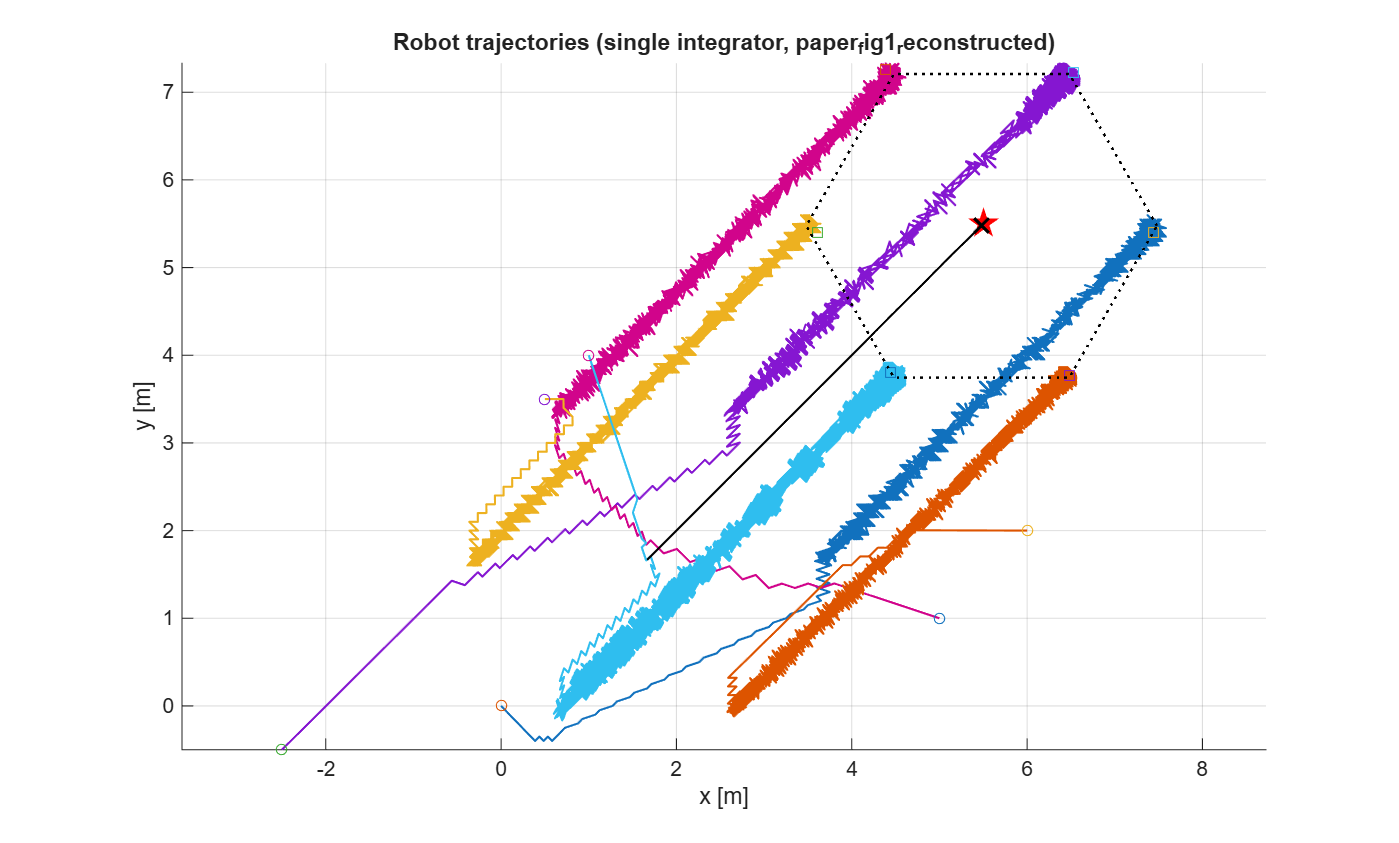
\includegraphics[width=0.48\textwidth]{sims/outputs/SingleIntegrator/trajectory.png}
\hfill
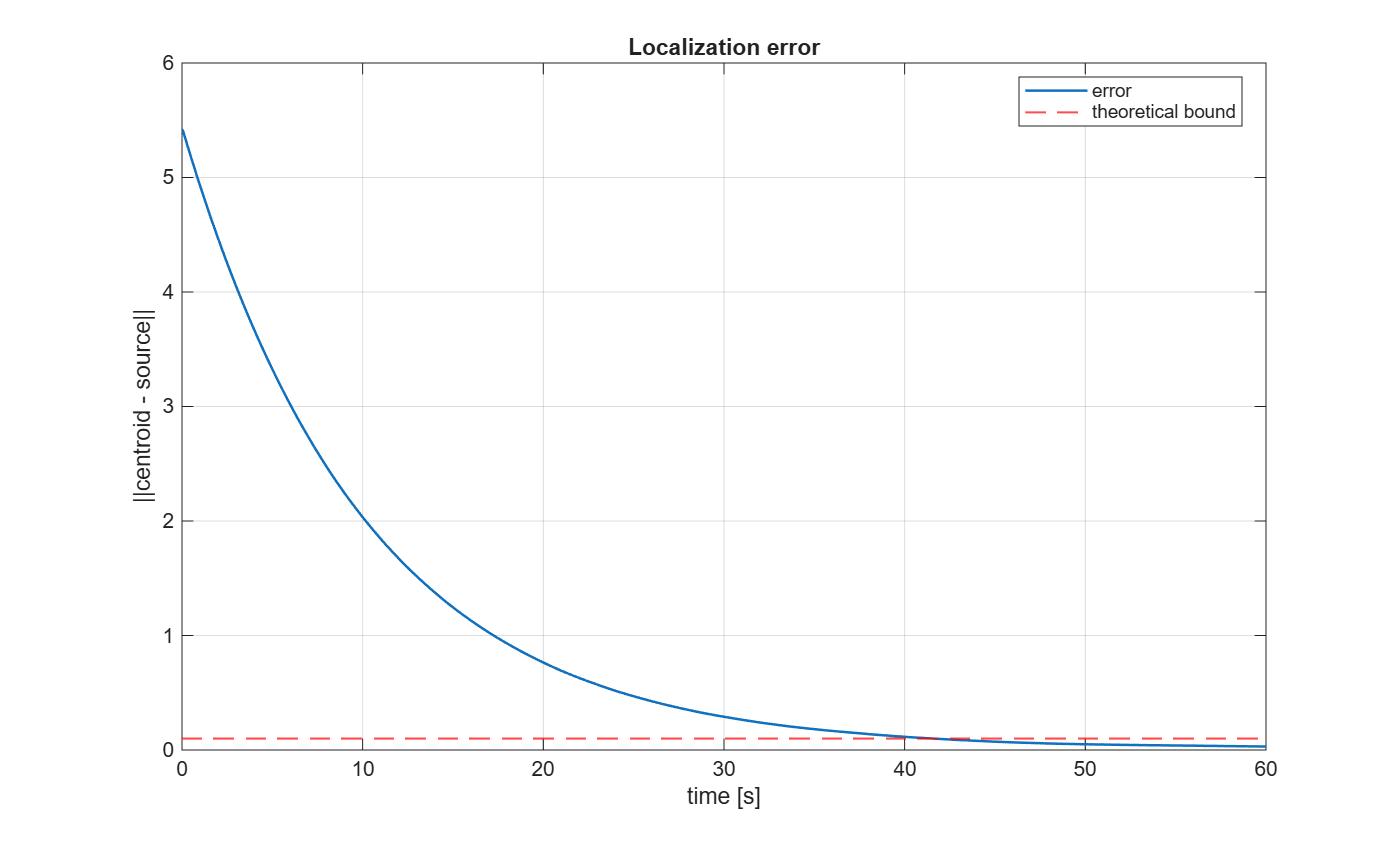
\includegraphics[width=0.48\textwidth]{sims/outputs/SingleIntegrator/localization_error.png}
\caption{Point robots. Left: the paths the six robots take, ending in an evenly spaced ring around
the source. Right: distance from the group centre to the source over time. It drops from about
$5.42$ to $0.030$, comfortably inside the predicted $0.1$.}
\label{fig:si}
\end{figure}

The formation term does its job almost immediately, within $0.025$~s, which is the finite-time
behaviour the theory promises. The localization error then decreases more slowly and enters the
predicted band at about $41.5$~s, staying inside it for the remaining $18.5$~s of the run.

One honest observation: the error does not settle to a perfectly flat line but keeps a small ripple.
The cause is the sign function. Near perfect formation the differences between robots are tiny and
keep crossing zero, so the sign flips between $-1$, $0$ and $+1$ very rapidly, and the fixed-step
integrator turns this into a small buzz. This is a property of simulating a discontinuous controller
with fixed time steps, not a flaw in the control law. It is quantified later in
Section~\ref{sec:checks}.

\subsection{Unicycle robots}

A real wheeled robot cannot slide sideways. It can drive forwards and it can turn, and that is all.
This is a unicycle. The control law of \eqref{eq:controller} asks for an arbitrary velocity vector,
which a unicycle usually cannot deliver.

The standard fix, which the paper also uses, is to stop steering the robot's centre and instead steer
a point a fixed distance $r$ in front of it. That offset point \emph{can} be moved in any direction,
so the original controller can be used unchanged and then converted into a forward speed and a turn
rate. This trick is called feedback linearization.

One extra change was needed in practice. Feeding a hard sign function into a turning robot produced
violent steering commands, because the sign flips instantly. Replacing the hard sign with a smooth
version inside a thin band around zero, a boundary layer of width $0.2$, removed the problem without
noticeably changing the behaviour.

\begin{figure}[H]
\centering
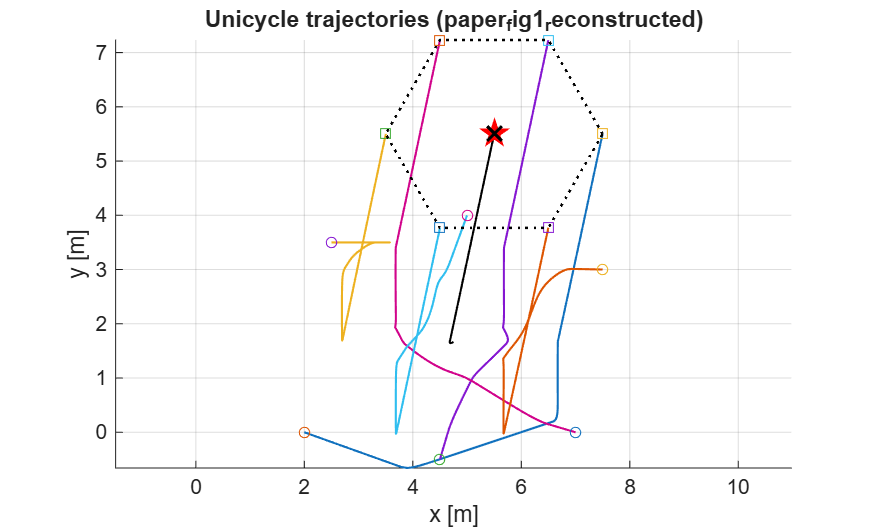
\includegraphics[width=0.48\textwidth]{sims/outputs/Unicycle/trajectory.png}
\hfill
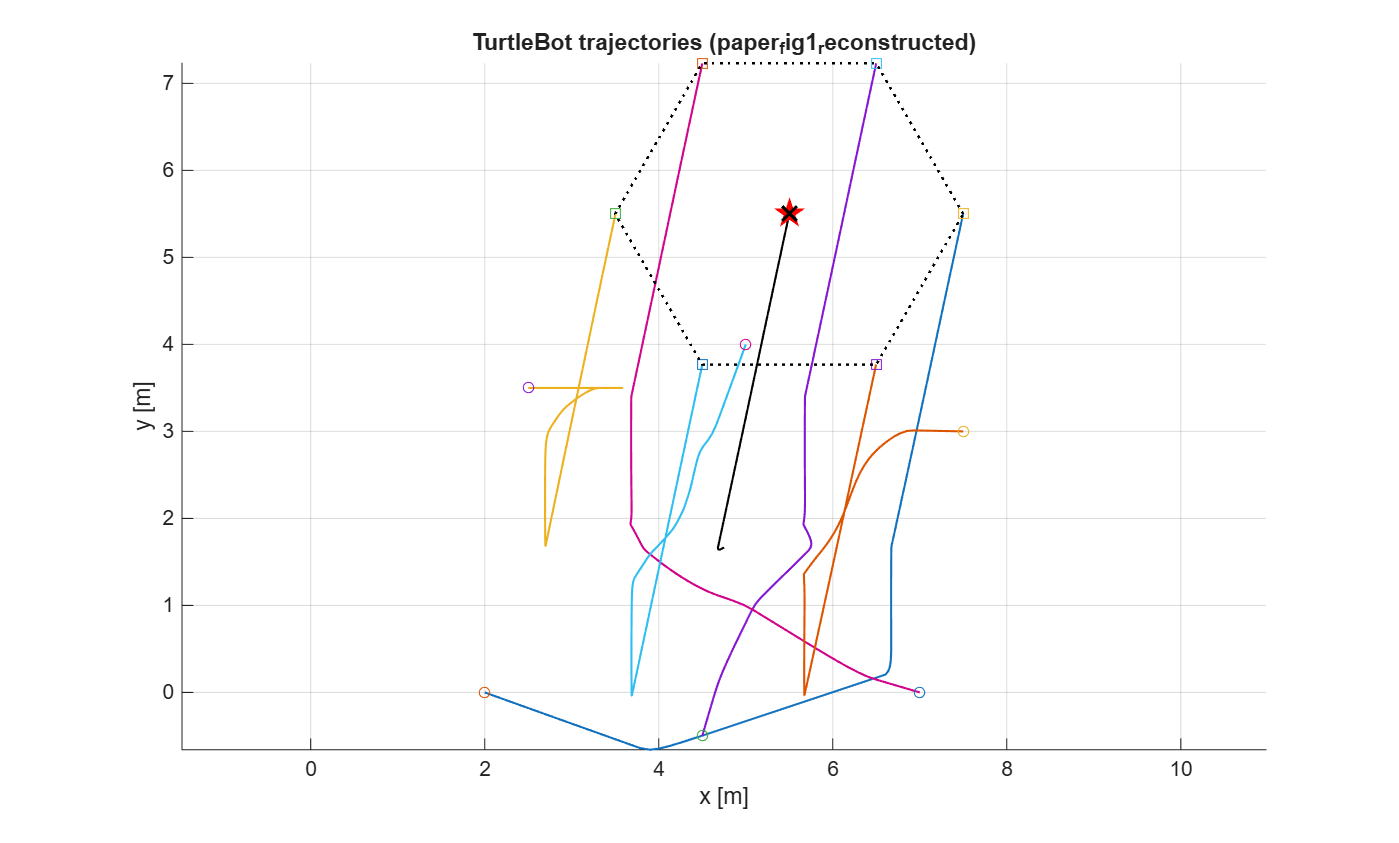
\includegraphics[width=0.48\textwidth]{sims/outputs/TurtleBot/trajectory.png}
\caption{Left: unicycle robots. Right: the same run with TurtleBot wheel geometry added. The final
paths are curved rather than straight, because these robots have to turn before they can go
somewhere.}
\label{fig:uni}
\end{figure}

The unicycle run ends with a localization error of $0.00089$, far inside the predicted $0.1$. It is
worth being careful about what that means. The gain ratio used here is $200$, which is
\emph{below} the theorem's sufficient threshold of about $1730$. So the theorem does not apply to
this run, and yet the result is excellent. That is not a contradiction: the threshold is a sufficient
condition, not a necessary one, so a run can succeed without meeting it. It does mean this run is
evidence that the controller works, not proof that the theorem holds.

\subsection{TurtleBot}

The last model adds the actual wheel geometry of a TurtleBot3: wheel radius $0.033$~m and wheel
separation $0.16$~m. The forward speed and turn rate are converted into left and right wheel speeds,
which is what a real robot's motors take as input.

The numbers come out identical to the unicycle run, which is the expected and correct result: the
wheels are a faithful re-parameterisation of the same motion, so nothing should change. What the
model \emph{does} add is a check on whether the commands are physically sensible. Here they are not
yet: the peak commanded speed is about $29.7$~m/s, whereas a real TurtleBot3 tops out near
$0.22$~m/s. Bringing the commands into a real robot's range is listed as future work in
Section~\ref{sec:future}.

\subsection{Summary of the reproduction}

\begin{table}[H]
\centering
\caption{Reproduction results. All three models finish well inside the predicted accuracy.}
\label{tab:baseline}
\small
\begin{tabular}{@{}lrrcc@{}}
\toprule
Model & Final error & Predicted $\varepsilon$ & Inside bound? & Gain condition met? \\
\midrule
Point robots & $0.0303$ & $0.1$ & yes & yes \\
Unicycle     & $0.00089$ & $0.1$ & yes & no \\
TurtleBot    & $0.00089$ & $0.1$ & yes & no \\
\bottomrule
\end{tabular}
\end{table}

The reproduction is therefore successful, with one caveat recorded honestly: the paper does not
publish its exact gains or its exact communication graph, so those had to be chosen. The graph used
is a reconstruction from the figure in the paper, and it is labelled as such throughout the code.

% ===========================================================================
\section{Part two: three gaps in the paper}

Once the reproduction worked, the natural question was what the method \emph{cannot} do. Three
limitations stood out, all of them following from assumptions the paper makes explicitly.

\begin{enumerate}
    \item The field is assumed to have \textbf{one} source. Real environments often have several.
    \item The source is assumed to be \textbf{stationary}. Leaks drift, vehicles move.
    \item The field is assumed to be a \textbf{single bowl}. A real field can have many peaks, and
    the method will happily settle on a small one.
\end{enumerate}

Each of the next three sections takes one of these, explains the idea, states what was proved, and
reports what the simulation measured.

% ===========================================================================
\section{Gap 1: many sources, many teams}

\subsection{The idea}

Suppose the field has $N$ sources instead of one. A robot's sensor reports the effect of whichever
source is nearest, so the field is a landscape of $N$ separate bowls. The plane divides naturally
into $N$ regions, one per source, where a region contains all the points closest to that source.
These regions are called Voronoi cells \cite{cortes2004}, and the borders between them are called
seams.

The plan is straightforward:

\begin{enumerate}
    \item Start all $n$ robots together as one group, moving towards the average of the sources.
    \item At a chosen time, split them into $N$ equal teams and assign each team to one source.
    \item Each team then runs the \emph{original, unchanged} algorithm on its own source.
\end{enumerate}

Starting together and splitting later, rather than splitting immediately, mirrors how a real
deployment would work: the swarm arrives as one unit and then fans out.

\subsection{How this compares with existing multi-source work}

Two existing methods were studied to check that this is a real gap rather than a solved problem. One
uses glowworm swarm optimization with distributed gradient estimation to capture several peaks at
once \cite{turgeman2018}. The other handles an unknown \emph{number} of sources in an unknown
environment \cite{chen2025dias}, which is a harder problem than the one addressed here.

Both are more capable than this work in terms of discovery: they do not need to be told how many
sources exist. Neither, however, provides what the approach here provides, namely a formation
guarantee and a stated accuracy radius per team, inherited directly from the original theorem. The
two lines of work are therefore complementary. A sensible combination would use a discovery method
to find how many sources there are and roughly where, and then hand over to the team-based scheme for
the precise, formation-holding endgame.

\subsection{What had to be proved}

Two results were needed, and one of them exposed a genuine weak point.

\textbf{Result one: team size does not help accuracy.} The natural assumption is that a bigger team
localizes better. It does not. Writing the paper's accuracy formula for a team of $n_k$ robots of
which a fraction $\chi_k$ can sense the source, the team size cancels out completely:
\begin{equation}\label{eq:teamscale}
    \varepsilon_k = \frac{2\pi\delta}{\kappa R_k \left( 2\pi\chi_k - \left|\sin(2\pi\chi_k)\right| \right)} .
\end{equation}
Only the \emph{fraction} of informed robots and the team's ring radius appear. The practical
consequence is direct: splitting twelve robots into three teams of four gives the same predicted
accuracy as splitting nine into three teams of three, provided the informed fraction and ring radius
match. If a twelve-robot run does look better, the reason is something else, such as a smoother
transient, and it should not be credited to the formula.

\textbf{Result two: teams must stay on their own side of the seam.} This is the weak point. Each
team's proof only works while all of its robots are inside their own region. But a team is a ring of
radius $R_k$, not a point, so a ring can cross a seam even when its centre has not. A condition was
written that can be checked while the simulation runs:
\begin{equation}\label{eq:certificate}
    \underbrace{\|p_k^* - p_s^{(k)}\|}_{\text{centre error}}
    + \underbrace{R_k}_{\text{ring radius}}
    + \underbrace{q_k}_{\text{formation error}}
    \;<\;
    \underbrace{d_k}_{\text{distance from source to seam}} .
\end{equation}
In words: the team's total reach must be smaller than the room it has. If this holds, every robot is
provably inside its own region and the original theorem applies to the team unchanged.

Being honest about the status of this result matters. The controller does not \emph{enforce}
\eqref{eq:certificate}; it only lets us check it. So the multi-source result is a conditional one:
it is correct whenever the condition holds, and the condition has to be reported for every run
rather than assumed. Closing that loop is genuine future work.

\subsection{What the simulation showed}

Three configurations were set up: eight robots with two sources, nine robots with three sources, and
twelve robots with three sources.

\begin{figure}[H]
\centering
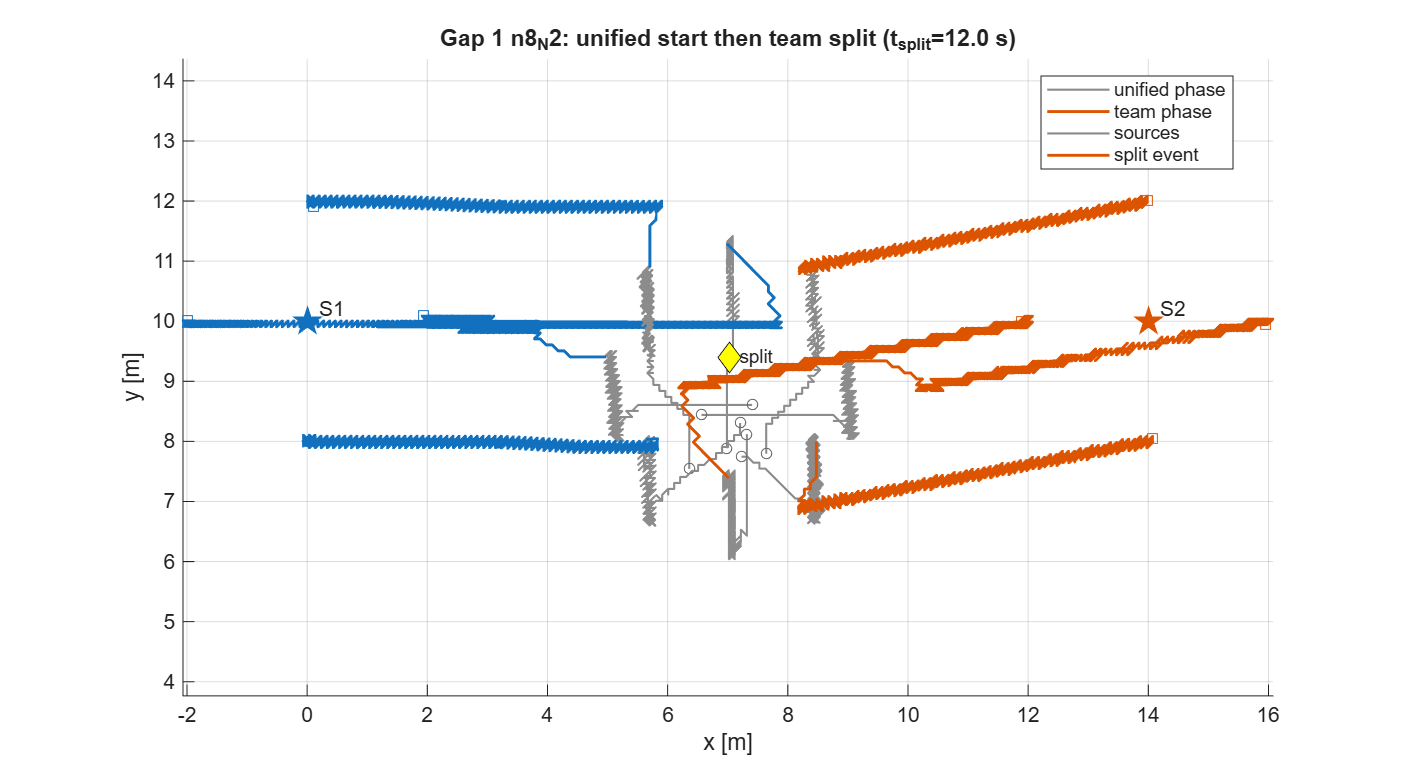
\includegraphics[width=0.48\textwidth]{sims/outputs/research/gap1/n8_N2/trajectory.png}
\hfill
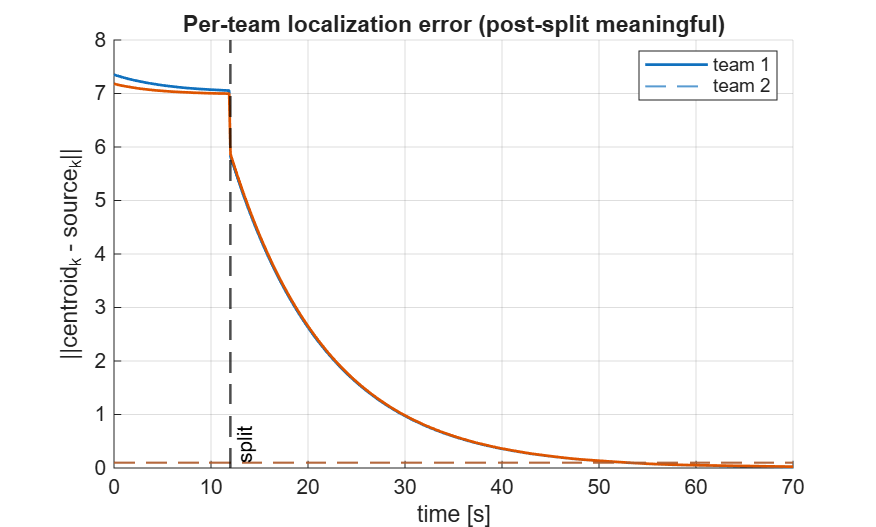
\includegraphics[width=0.48\textwidth]{sims/outputs/research/gap1/n8_N2/team_localization.png}
\caption{Eight robots, two sources. Left: the swarm starts as one cluster near the centre, then
splits and fans out to the two sources. Right: each team's distance to its own source, both settling
inside the predicted band.}
\label{fig:gap1a}
\end{figure}

\begin{figure}[H]
\centering
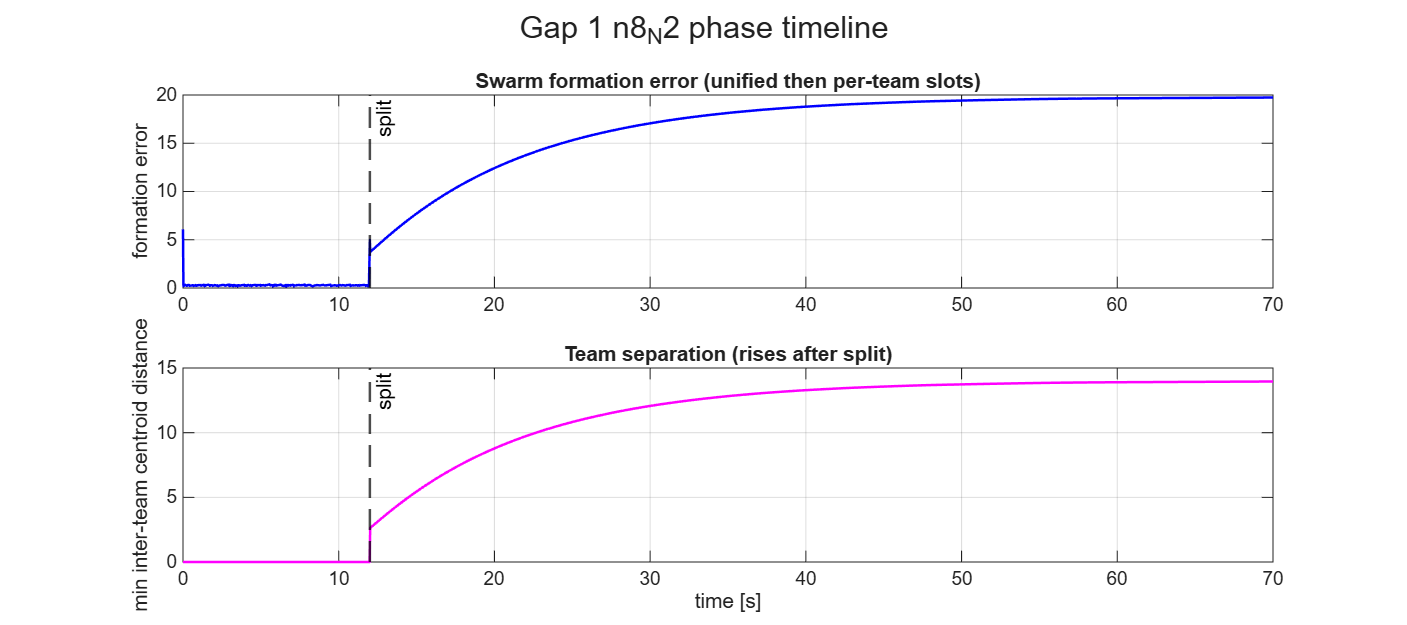
\includegraphics[width=0.48\textwidth]{sims/outputs/research/gap1/n8_N2/phase_timeline.png}
\hfill
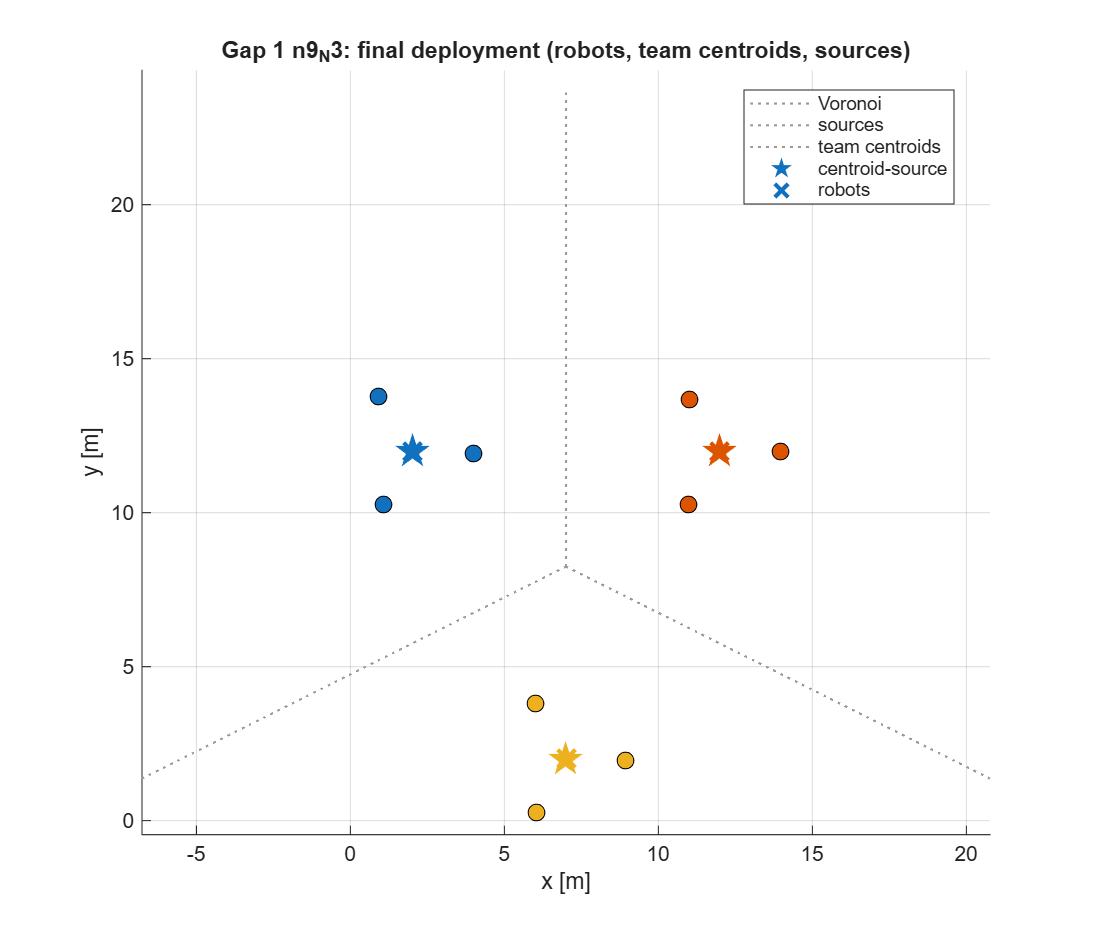
\includegraphics[width=0.48\textwidth]{sims/outputs/research/gap1/n9_N3/deployment_map.png}
\caption{Left: the timeline of the eight-robot run, showing the unified phase, the split, and the
settled phase. Right: the final deployment for nine robots and three sources, with each team of
three surrounding its own source.}
\label{fig:gap1b}
\end{figure}

For the eight-robot, two-source run the two teams finish at distances $0.0195$ and $0.0249$ from
their sources, against a predicted $0.1$ each, so both are inside the bound. The teams end up
$13.96$ apart, confirming they genuinely separated rather than drifting towards each other.

One number in the output file is easy to misread. The overall formation error for this run is
$19.74$, which looks like a failure. It is not. That number measures how far the robots are from a
\emph{single} common ring, and after the split there is no single ring: there are two rings far
apart. The meaningful quantities after the split are the per-team numbers, which are the ones quoted
above. This is exactly the sort of thing that only becomes obvious once you have run the simulation
and stared at the output.

Status note for completeness: the eight-robot, two-source configuration has been run end to end with
its numbers recorded. The nine-robot run has produced its figures, and the twelve-robot
configuration is defined in the code but has not yet been run to completion. Finishing both is
listed in Section~\ref{sec:future}.

% ===========================================================================
\section{Gap 2: a source that keeps moving}

\subsection{The idea}

If the source moves, the robots can never sit exactly on it. They will always be a little behind.
The useful question is not whether there is an error but \emph{how big} it is and \emph{what it
depends on}.

\subsection{What had to be proved}

Three results, and the first one is the reason this problem has a clean answer.

\textbf{The formation does not care that the source is moving.} Working through the formation
argument, the source's velocity never appears anywhere. The only thing the formation term needs from
the measurement is that it stays bounded in size, and that is true whether the source sits still or
moves. So the finite-time formation guarantee carries over with no changes at all.

\textbf{Source motion is just a disturbance.} With the ring exact, the error $e$ between the group
centre and the source obeys
\begin{equation}\label{eq:movingdyn}
    \dot e = -\lambda e + d_\eta - \dot p_s,
    \qquad \lambda = 2\beta\kappa .
\end{equation}
Read this as three effects. The $-\lambda e$ term pulls the error towards zero. The $d_\eta$ term is
sensor noise. The $-\dot p_s$ term is the source running away. Structurally the source's motion is
just one more push on a system that was already stable, which is why no redesign is needed.

\textbf{The error settles inside a known radius.} Combining the two pushes gives
\begin{equation}\label{eq:movingbound}
    \limsup_{t\to\infty} \| e(t) \|
    \;\leq\;
    \underbrace{\frac{\delta}{\kappa R}}_{\text{noise, same as before}}
    \;+\;
    \underbrace{\frac{v_{\max}}{2\beta\kappa}}_{\text{price of motion}} .
\end{equation}
The first term is exactly the stationary-source accuracy from \eqref{eq:epsilon}. The second is new
and is the cost of the source moving. Notice that $\beta$ does not appear in the first term but does
appear in the second: turning up $\beta$ shrinks the motion penalty without making the noise floor
worse. That is a concrete design rule that falls straight out of the algebra.

\textbf{For a source moving at constant velocity, the lag is exactly predictable.} If the source
moves with a fixed velocity $v$ and there is no noise, the error converges to the specific vector
\begin{equation}\label{eq:lag}
    e_\infty = -\frac{v}{2\beta\kappa} .
\end{equation}
This is a sharper statement than \eqref{eq:movingbound}, because it fixes both the size \emph{and}
the direction of the lag, and a two-component prediction is much harder to satisfy by accident.

A useful consequence follows if an estimate of the source velocity is available: adding the same
estimated velocity to every robot's command cancels out of the formation dynamics entirely, because
it is common to all robots, while shrinking the motion penalty in \eqref{eq:movingbound}. A perfect
estimate recovers the stationary accuracy exactly. Building a distributed estimator that supplies it
is a separate problem, and gradient-free seeking of a moving source under different structural
assumptions is treated in \cite{michael2023}.

\subsection{What the simulation showed}

The run uses six robots and a source drifting at velocity $(0.03, 0.02)$, so a speed of about
$0.036$. Formula \eqref{eq:movingbound} predicts a settling radius of $0.461$.

\begin{figure}[H]
\centering
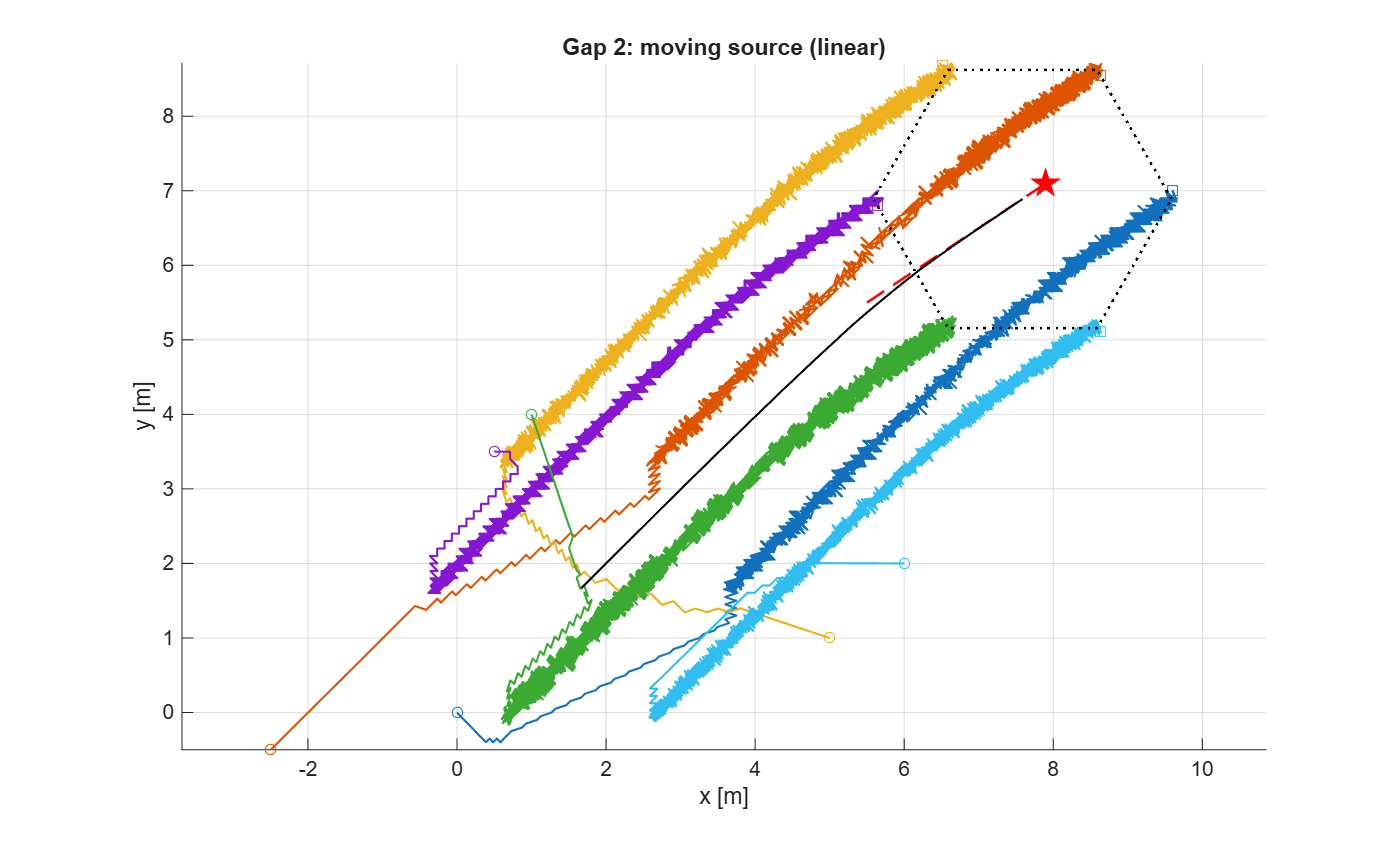
\includegraphics[width=0.48\textwidth]{sims/outputs/research/gap2/trajectory.png}
\hfill
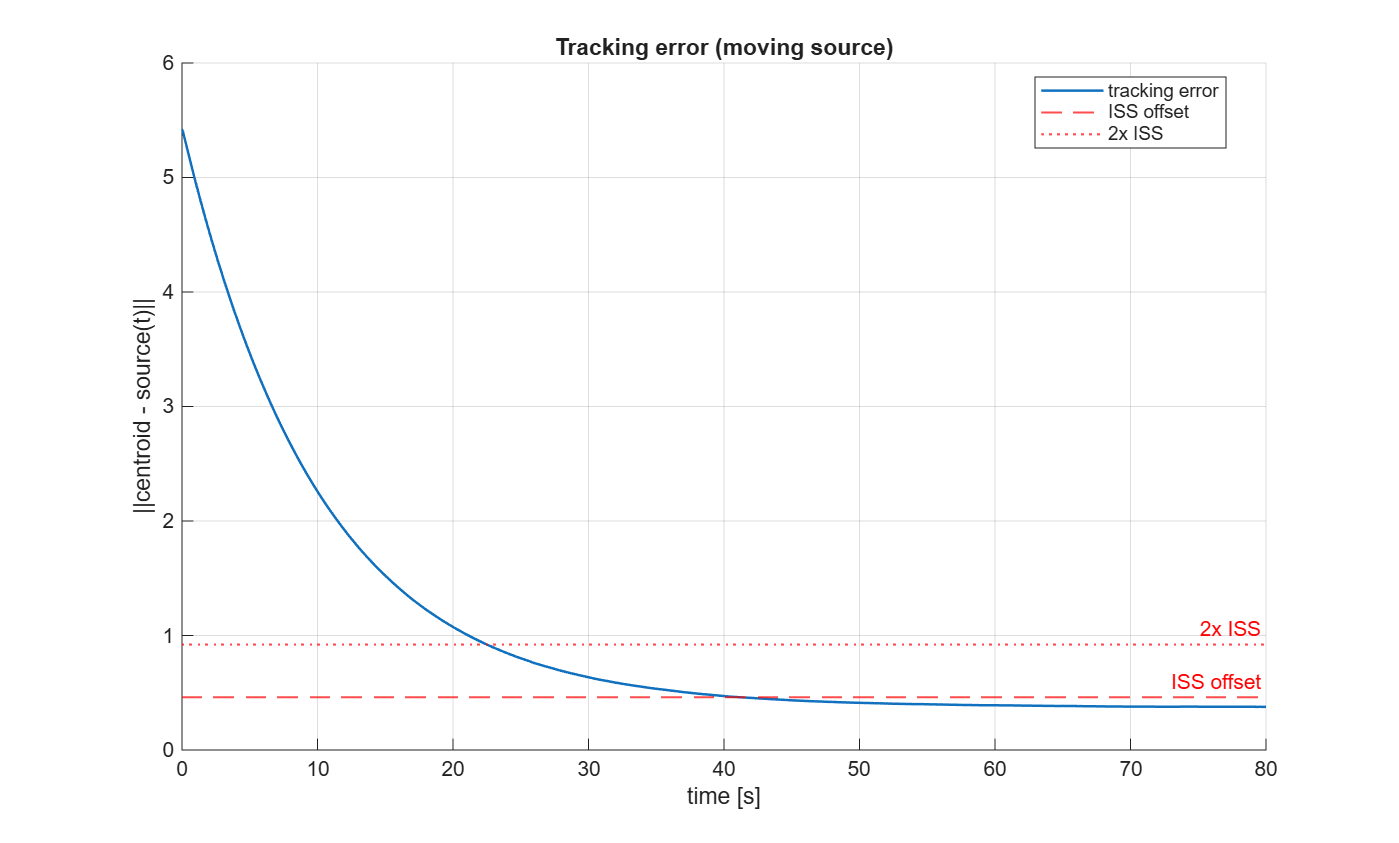
\includegraphics[width=0.48\textwidth]{sims/outputs/research/gap2/localization_error.png}
\caption{Moving source. Left: the robots chase the drifting source and then travel alongside it in
formation. Right: the tracking error, which does not go to zero but flattens out at a steady lag, as
predicted.}
\label{fig:gap2}
\end{figure}

The error peaks at $5.43$ while the robots are still catching up, then settles at $0.377$ with a
tail average of $0.381$. Both are below the predicted $0.461$, so the bound holds and is
reasonably tight, roughly $82\%$ of the prediction. The characteristic shape of the plot is the
result worth noting: the error stops decreasing and levels off at a non-zero value. That is a
moving-source signature and cannot happen for a stationary source.

The direction of the lag was tested separately and matched the prediction of \eqref{eq:lag} to
$2.3\%$ on both components.

% ===========================================================================
\section{Gap 3: many peaks, one true peak}

\subsection{The idea}

Real fields are lumpy. A field with three peaks of different heights has one true global maximum and
two decoys. Any method that only ever climbs uphill will stop at whichever peak it happens to be
near, and will then report success. The two questions are: how bad is this, and what can be done?

\subsection{What had to be proved}

\textbf{Getting stuck is unavoidable, and it is not a rare accident.} Around any local peak there is
a whole region of starting points from which the robots will climb to \emph{that} peak and stop.
Using the field value itself as an energy function shows the region is an open set with genuine area,
not a thin exceptional sliver. So no amount of gain tuning fixes this. Escaping needs a mechanism
that is not pure local hill-climbing.

\textbf{The ring's gradient estimate has a bias, and it depends sharply on the number of robots.}
On a curved, non-bowl-shaped field the ring no longer recovers the gradient exactly. The leftover
error is small, proportional to $R^2$, provided $n \geq 4$. At $n = 3$ a third identity that the
proof relies on fails, and the error becomes proportional to $R$ instead, which is an entire order
worse. This is a real design rule: use at least four robots per team.

\textbf{Running several teams and picking the best one works, under a stated condition.} If $M$
teams are launched from different places, each ends near some peak and reports its score. Picking the
highest score is guaranteed to pick a team that found the global peak, provided
\begin{equation}\label{eq:selection}
    \Delta > 2\left( L_f \varepsilon_{\mathrm{loc}} + \delta_F \right),
\end{equation}
where $\Delta$ is the height gap between the best and second-best peak, $\varepsilon_{\mathrm{loc}}$
is how far a team stops from its peak, and $\delta_F$ is the error in the reported score. Plainly:
the peaks must be more clearly separated in height than the total measurement sloppiness. The
factor of two says positional error and score error are equally damaging.

\subsection{What the simulation showed}

The test field has three peaks of heights $5$, $2$ and $1.5$. The robots start near a small peak.

\begin{figure}[H]
\centering
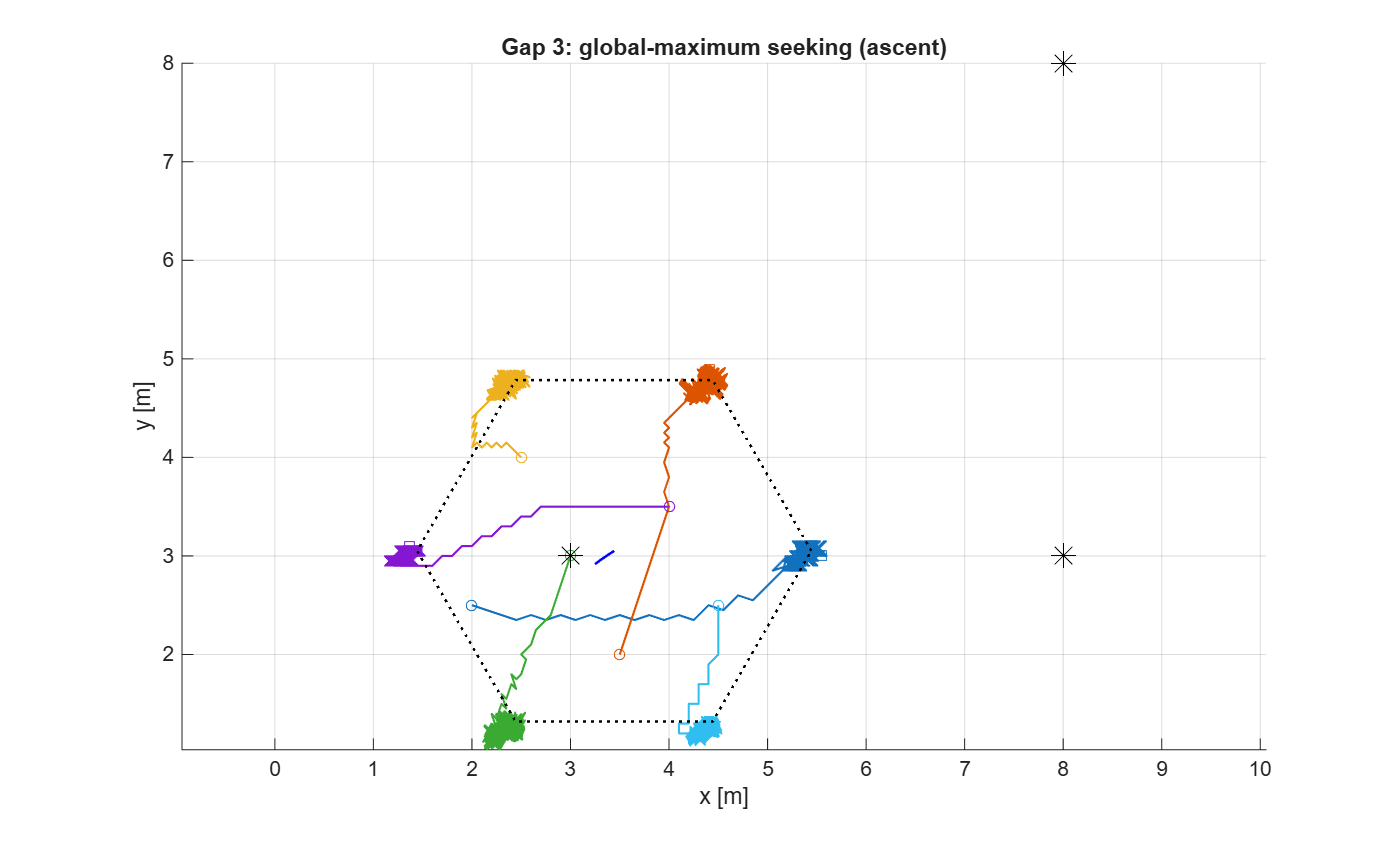
\includegraphics[width=0.48\textwidth]{sims/outputs/research/gap3/trajectory.png}
\hfill
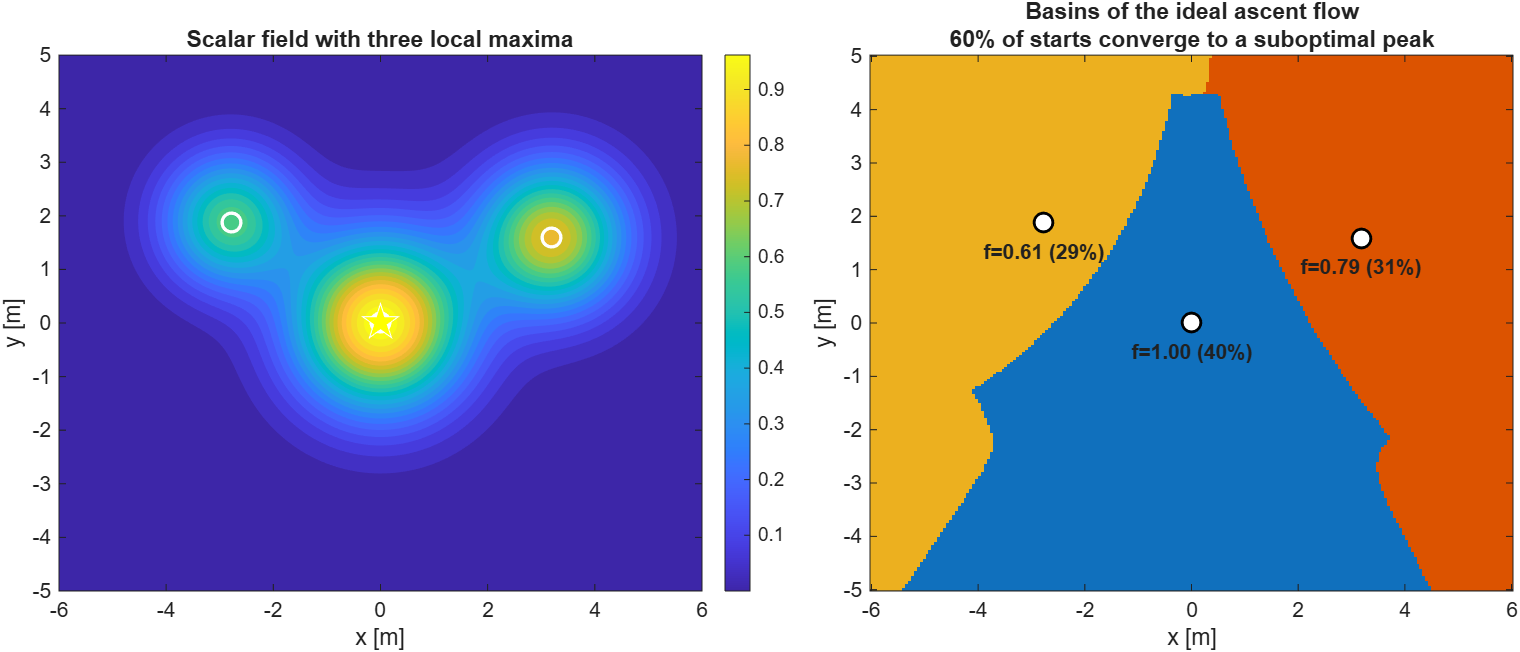
\includegraphics[width=0.48\textwidth]{sims/outputs/verify_theory/v11_local_trapping.png}
\caption{Left: single-start hill climbing on a three-peak field. The robots settle on a small peak
and stop. Right: the same field coloured by which peak the robots end up at, for $48\,400$ different
starting points. The two suboptimal peaks together claim $60\%$ of them.}
\label{fig:gap3}
\end{figure}

The single run ends at a field value of $2.08$ out of a possible $5$, that is $42\%$ of the global
maximum, sitting $0.45$ away from the wrong peak. It reports \texttt{reached\_global\_peak: false}.

This is a \textbf{successful} test, not a failure. The theory predicts getting stuck, and the
simulation gets stuck. What makes it convincing rather than anecdotal is the sweep in the right
panel: across $48\,400$ starting points, $60\%$ end at a suboptimal peak. So getting trapped is the
normal case on this field, not bad luck. That is the quantitative justification for treating
multiple restarts as a requirement rather than an optional improvement.

The selection rule \eqref{eq:selection} was tested separately over a grid of error sizes with
$4\,000$ trials per point. Everywhere the condition holds, selection was correct $100\%$ of the time.
Outside the condition it degrades gently, still $97.7\%$ at the widest errors tried, which tells us
the condition is conservative: it is a worst-case guarantee, not a prediction of where things break.

% ===========================================================================
\section{Checking the mathematics with plots}
\label{sec:checks}

Algebra can be wrong and still look fine. To guard against that, a separate script was written that
turns each mathematical claim into a plot comparing a measured quantity against the predicted one.
Each check is designed as an attempt to \emph{break} the claim, so that a wrong claim shows up as a
visibly wrong curve rather than a silent pass. There are fourteen checks and all fourteen pass; the
full suite takes about four minutes.

\begin{table}[H]
\centering
\caption{The fourteen verification checks and their outcomes.}
\label{tab:checks}
\small
\begin{tabular}{@{}llp{0.44\linewidth}@{}}
\toprule
ID & What it tests & Outcome \\
\midrule
V1 & Slot-direction identities & Exact for $n \geq 4$; fails at $n = 3$ as expected \\
V2 & A comparison inequality & $600/600$ random graphs satisfy it \\
V3 & Finite-time formation & Settles two decades before the predicted deadline \\
V4 & Exact gradient recovery & Machine precision on the bowl-shaped field \\
V5 & Accuracy bound & Worst tail error $0.0148$ against a bound of $0.05$ \\
V6 & Internal consistency of the formula & Constant to $1.7 \times 10^{-16}$ \\
V7 & Team size cancels & Flat in team size to $5.6 \times 10^{-16}$ \\
V8 & Seam-crossing condition & Sufficiency respected; tight case loses containment \\
V9 & Moving-source lag & Lag vector matches to $2.3\%$ \\
V10 & Gradient-estimate bias & Slope $1.10$ at $n=3$, $1.99$ for $n \geq 4$ \\
V11 & Getting stuck on local peaks & Suboptimal peaks claim $60\%$ of the domain \\
V12 & Multi-team selection rule & $100\%$ correct inside the guaranteed region \\
V13 & A condition that is never needed & Positive everywhere; worst case $1.15\times10^{-2}$ \\
V14 & Exact bias formula at $n=3$ & Size matches to $0.002\%$, direction to $0.015^\circ$ \\
\bottomrule
\end{tabular}
\end{table}

Four of these deserve individual mention, because each one changed something.

\textbf{V3 found a measurement floor in our own simulation.} The theory says the formation error
goes to exactly zero. In simulation it does not: it settles at a small non-zero level caused by the
sign function chattering between time steps. Sweeping the step size confirmed that this floor is
proportional to the step size. At the settings used for the gap runs it sits near $0.15$. That is a
directly useful piece of self-knowledge: any reported formation error below about $0.15$ is a
simulation artefact and must not be presented as a real result.

\begin{figure}[H]
\centering
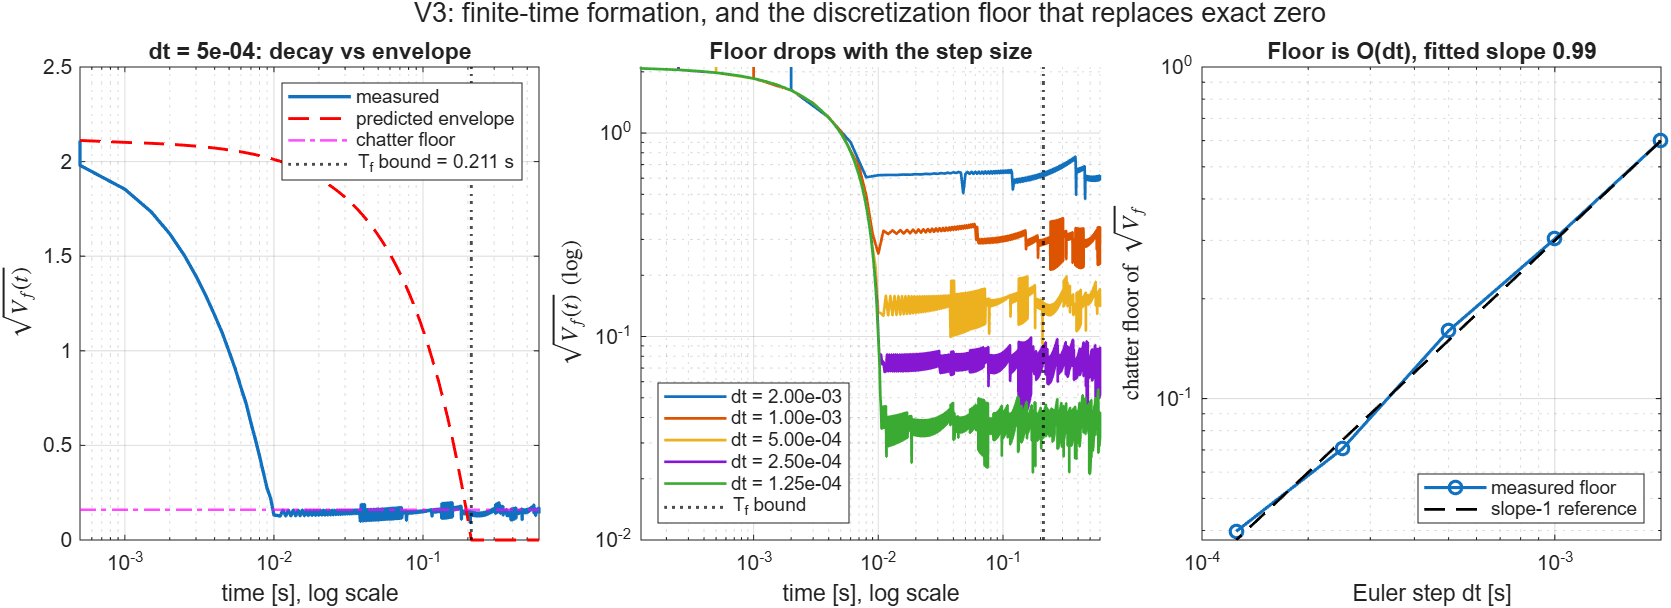
\includegraphics[width=0.72\textwidth]{sims/outputs/verify_theory/v3_formation_finite_time.png}
\caption{V3. Left: the formation error decays far faster than the guaranteed deadline, then stops at
a floor. Right: that floor scales with the integration step size, confirming it is a numerical
artefact rather than a property of the control law.}
\label{fig:v3}
\end{figure}

\textbf{V8 showed the seam condition is not a formality.} Two cases were run. With sources far apart
the condition holds and the teams stay in their own regions. With sources close together, where the
ring radius alone almost uses up the available room, the condition fails \emph{and} containment is
genuinely lost during the transient. So crossing a seam is a real failure mode, which is why
\eqref{eq:certificate} has to be logged for every run.

\begin{figure}[H]
\centering
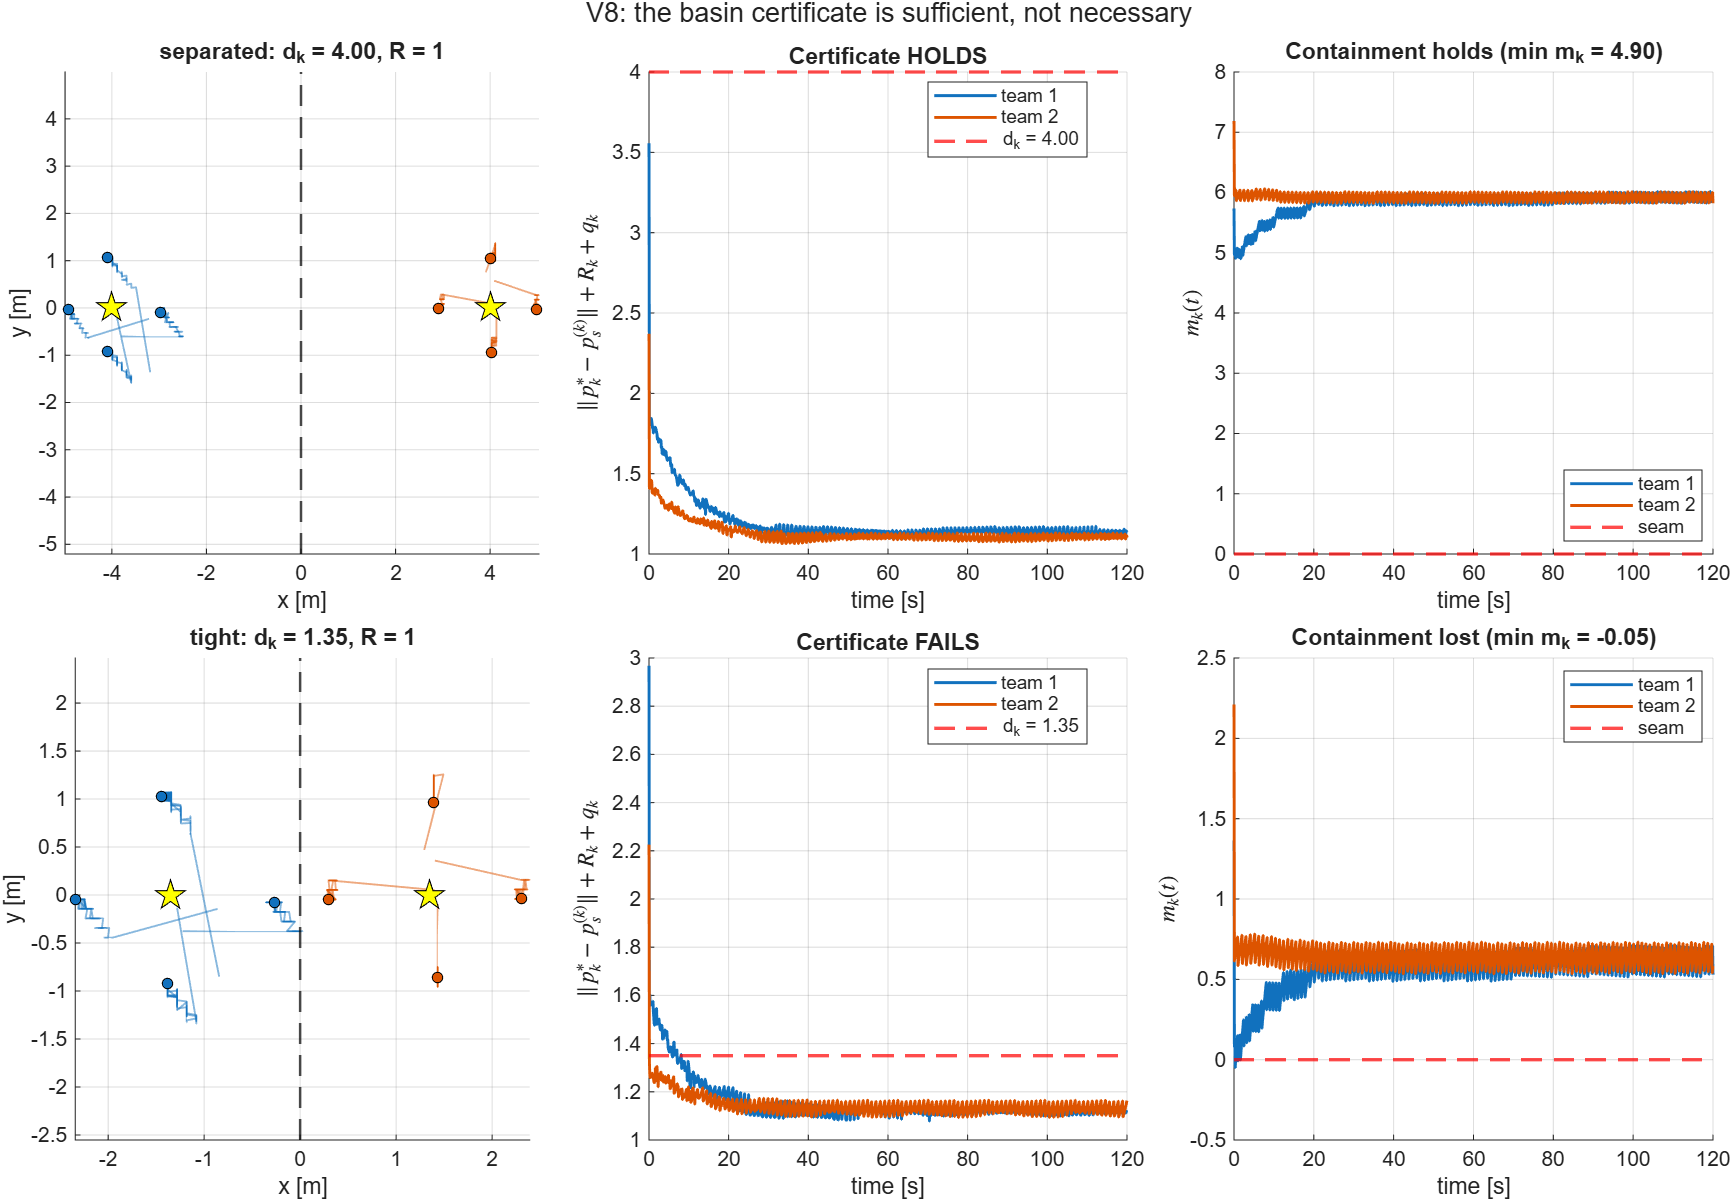
\includegraphics[width=0.85\textwidth]{sims/outputs/verify_theory/v8_basin_certificate.png}
\caption{V8. Top row, sources far apart: condition holds and containment holds. Bottom row, sources
close together: condition fails and containment is genuinely lost.}
\label{fig:v8}
\end{figure}

\textbf{V10 pinned down what ``at least four robots'' actually buys.} Fitting the bias against ring
radius on a log-log scale gives slope $1.99$ for $n = 4, 6, 8$ and slope $1.10$ for $n = 3$. The
difference is a full order in $R$, not a constant factor.

\textbf{V14 turned an excluded case into a formula.} V10 established only that the $n = 3$ bias
behaves like $R$. Working out what actually survives the algebra gives the exact leading term
\begin{equation}\label{eq:n3bias}
    \| r_R \| = \frac{R}{4}\sqrt{\left(H_{11} - H_{22}\right)^2 + 4H_{12}^2} + O(R^2),
\end{equation}
where $H$ is the field's curvature matrix at that point. The measurement agrees to $0.002\%$ in size
and $0.015^\circ$ in direction. In plain terms, a three-robot ring points slightly the wrong way
whenever the field is curved differently in different directions, and that error shrinks only
linearly with the ring size. Since a small ring also means worse noise rejection, this is a real
trade-off, and using four or more robots removes it entirely.

\begin{figure}[H]
\centering
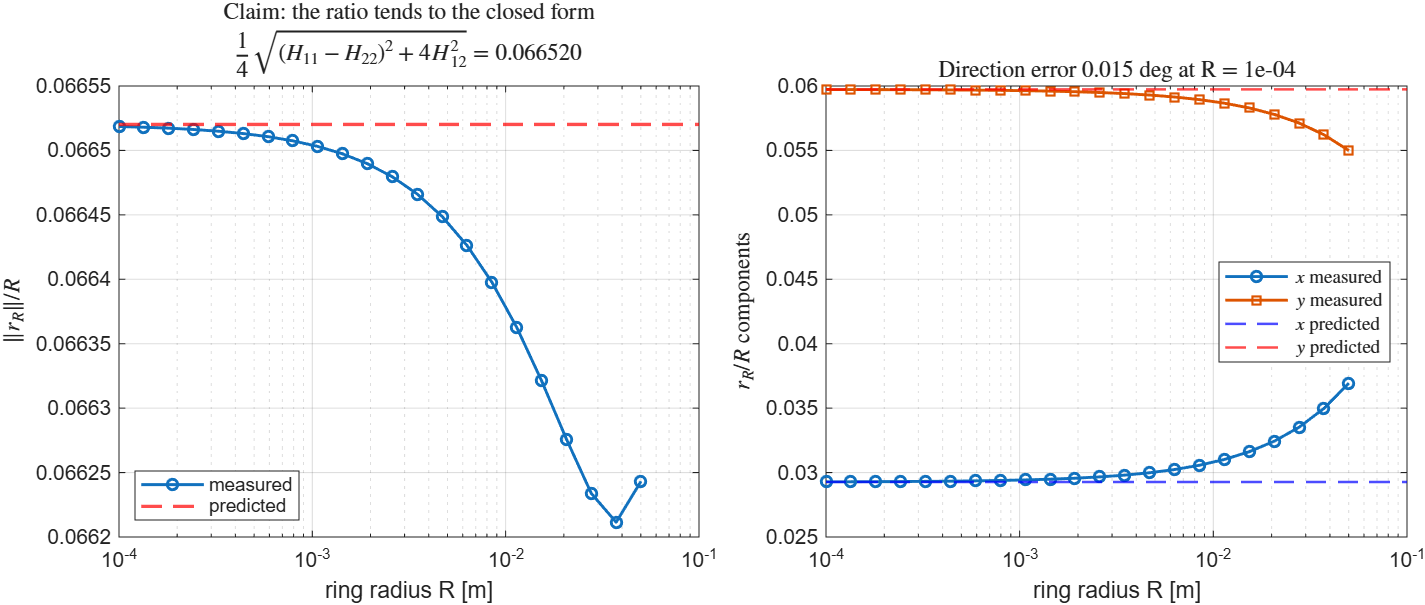
\includegraphics[width=0.85\textwidth]{sims/outputs/verify_theory/v14_n3_bias_constant.png}
\caption{V14. Left: the measured bias per unit radius converges to the closed-form constant. Right:
both components of the bias vector converge to their predicted values, so the direction is confirmed
and not just the magnitude.}
\label{fig:v14}
\end{figure}

Two of these results, V13 and V14, were not in the original plan. They appeared only while writing
the proofs out step by step for the theory document, which is the strongest argument I encountered
during the internship for writing proofs in full rather than in outline.

% ===========================================================================
\section{Written theory documents}

Two LaTeX documents were produced alongside the code.

\begin{itemize}
    \item A \textbf{research note} presenting the three gaps with their mathematical framing, related
    work, the verification figures embedded beside the claims they support, and a validation plan.
    Every statement is labelled as established, conditional, or proposed, so a reader can tell at a
    glance how much weight it carries.
    \item A \textbf{proofs-only companion} covering the same three gaps with every algebraic step
    written out and numbered, together with tables of predicted-versus-measured numbers.
\end{itemize}

Because no LaTeX compiler was available on the machine used, a small Python checker was written to
catch the errors a compiler would normally catch: unbalanced delimiters, references pointing at
labels that do not exist, citations without bibliography entries, unbalanced environments, and table
rows with the wrong number of columns. A second script deliberately injects known faults into a copy
of the document and confirms the checker reports each one, so the checker itself is tested rather
than trusted. Both documents pass cleanly.

% ===========================================================================
\section{Limitations, stated honestly}

An internship report is more useful if it says what is not settled. The following are open.

\begin{enumerate}
    \item \textbf{The multi-source result is conditional.} The seam condition \eqref{eq:certificate}
    is checkable but not enforced by the controller. In particular the proof needs the condition to
    hold during the transient right after the split, which is exactly when the formation error is
    largest. Closing this needs either a bound on that transient or a controller that keeps robots
    inside their region by construction.
    \item \textbf{The multi-source runs use labelled measurements.} After the split, each robot is
    told which source its reading belongs to. That makes the setup an experiment in \emph{deploying}
    teams to known sources, not an algorithm that \emph{discovers} an unknown number of sources on
    its own.
    \item \textbf{Two Gap 1 configurations are not finished.} The eight-robot, two-source case is
    complete with recorded numbers. The nine-robot case has figures, and the twelve-robot case has
    not been run.
    \item \textbf{Escaping local peaks is not solved.} The selection rule tells us how to
    \emph{recognise} the global peak once several teams have reported. It does not tell us how to
    guarantee that some team lands in the right region in the first place.
    \item \textbf{The bounds are loose.} Several results are upper bounds obtained through triangle
    inequalities, so they are correct but conservative. V5 and V12 both show measured behaviour well
    inside the guarantee. Loose bounds should not be quoted as predictions of what will be observed.
    \item \textbf{Commanded speeds are not yet physical.} The TurtleBot model reproduces the wheel
    geometry but the commands exceed a real TurtleBot3's limits by two orders of magnitude.
    \item \textbf{The reproduction involves reconstructed inputs.} The paper does not publish its
    gains or its communication graph numerically, so both were chosen and are documented as choices.
    \item \textbf{Simulation only.} No result in this report has been tested on hardware.
\end{enumerate}

% ===========================================================================
\section{What I learned}

\textbf{Reproducing before extending is worth the time.} Rebuilding the paper first meant that when
the extensions misbehaved, the baseline could be trusted, and the fault was always in the new part.

\textbf{Check against theorems, not against pictures.} It is easy to produce a plot that resembles a
published figure and conclude the implementation is right. Checking the gain condition and the
accuracy bound numerically is a much stronger test, and it caught real issues.

\textbf{Know your own simulator's noise floor.} The V3 result, that formation error cannot go below
roughly the step size times the gain, changed how every later result was reported. Without it I would
have quoted meaningless numbers with confidence.

\textbf{Writing proofs in full finds things.} The two new results in this report, V13 and V14, both
appeared while expanding an argument that had previously been written in outline. In one case an
assumption everyone carries around turned out never to be needed; in the other, an excluded special
case turned out to have a clean exact formula.

\textbf{State the status of every claim.} Distinguishing established from conditional from proposed
is not bureaucracy. It stops a conditional result from quietly being cited later as though it were
proved.

\textbf{Build the same thing twice when you can.} Having Python and MATLAB implementations of the
same model made it easy to tell coding mistakes apart from genuine behaviour.

% ===========================================================================
\section{Future work}
\label{sec:future}

\begin{enumerate}
    \item Finish the remaining two Gap 1 configurations and record their numbers alongside the
    eight-robot case.
    \item Bound the formation error during the post-split transient, which would upgrade the
    multi-source result from conditional to unconditional.
    \item Replace the labelled measurements with genuine source discovery, so the number of sources
    does not have to be known in advance.
    \item Design a distributed estimator for the source velocity. The theory already shows that
    feeding such an estimate forward shrinks the moving-source penalty, and a perfect estimate
    recovers the stationary accuracy exactly.
    \item Investigate dither for escaping local peaks, in the spirit of extremum seeking control
    \cite{krsticwang2000,khong2014}. This is currently a hypothesis with no proof: the standard
    averaging results are local around an averaged equilibrium, and matching them to a decaying
    dither schedule on a multi-peak field needs assumptions about barrier widths and depths that are
    not yet available.
    \item Bring the commanded velocities inside real TurtleBot3 limits and re-verify the bounds under
    saturation.
    \item Compile both theory documents once a LaTeX toolchain is available, since they have so far
    only been checked statically.
\end{enumerate}

% ===========================================================================
\section{Conclusion}

The internship reproduced a 2024 distributed control result from scratch and verified it against its
own theorems rather than its figures, across three robot models of increasing realism. All three
finish inside the accuracy the theory predicts.

Building on that, three limitations of the original method were identified and worked through. For
multiple sources, the robots can split into teams and each team runs the unchanged algorithm,
provided a checkable seam condition holds; a side result is that team size does not improve accuracy,
only the informed fraction and ring radius do. For a moving source, the formation guarantee survives
untouched and the tracking error settles at a predictable lag whose size and direction were both
confirmed. For a multi-peak field, getting trapped was shown to be the normal outcome rather than
bad luck, affecting $60\%$ of starting points on the test field, and a rule was proved for
recognising the true global peak once several teams report.

All fourteen mathematical claims have a numerical check behind them, and all fourteen pass. Two new
results emerged from writing the proofs out completely. The parts that remain unproved are stated as
such rather than smoothed over, which I have come to see as the most useful habit the internship
taught me.

% ===========================================================================
\begin{thebibliography}{9}

\bibitem{du2024}
Y.~Du, F.~Chen, L.~Xiang, G.~Guo, and G.~Chen,
``Simultaneous source localization and formation via a distributed sign gradient-free algorithm,''
\emph{IEEE Transactions on Control of Network Systems}, vol.~11, no.~1, pp.~319--327, Mar.~2024.
doi: \href{https://doi.org/10.1109/TCNS.2023.3281369}{10.1109/TCNS.2023.3281369}.

\bibitem{animations}
\studentname, ``Simulation animations (GIF) for this report,'' shared drive folder.
Available: \expandafter\url\expandafter{\drivelink}

\bibitem{cortes2004}
J.~Cort\'es, S.~Mart\'inez, T.~Karata\c{s}, and F.~Bullo,
``Coverage control for mobile sensing networks,''
\emph{IEEE Transactions on Robotics and Automation}, vol.~20, no.~2, pp.~243--255, 2004.
doi: \href{https://doi.org/10.1109/TRA.2004.824698}{10.1109/TRA.2004.824698}.

\bibitem{michael2023}
E.~Michael, C.~Manzie, T.~A.~Wood, D.~Zelazo, and I.~Shames,
``Gradient free cooperative seeking of a moving source,''
\emph{Automatica}, vol.~152, art.~110948, 2023.
doi: \href{https://doi.org/10.1016/j.automatica.2023.110948}{10.1016/j.automatica.2023.110948}.

\bibitem{khong2014}
S.~Z.~Khong, Y.~Tan, C.~Manzie, and D.~Ne\v{s}i{\'c},
``Multi-agent source seeking via discrete-time extremum seeking control,''
\emph{Automatica}, vol.~50, no.~9, pp.~2312--2320, 2014.
doi: \href{https://doi.org/10.1016/j.automatica.2014.06.009}{10.1016/j.automatica.2014.06.009}.

\bibitem{krsticwang2000}
M.~Krsti{\'c} and H.-H.~Wang,
``Stability of extremum seeking feedback for general nonlinear dynamic systems,''
\emph{Automatica}, vol.~36, no.~4, pp.~595--601, 2000.
doi: \href{https://doi.org/10.1016/S0005-1098(99)00183-1}{10.1016/S0005-1098(99)00183-1}.

\bibitem{turgeman2018}
A.~Turgeman and H.~Werner,
``Multiple source seeking using glowworm swarm optimization and distributed gradient estimation,''
in \emph{Proc. American Control Conference (ACC)}, Milwaukee, WI, USA, 2018, pp.~3558--3563.
doi: \href{https://doi.org/10.23919/ACC.2018.8431479}{10.23919/ACC.2018.8431479}.

\bibitem{chen2025dias}
L.~Chen, S.~Kailas, S.~Deolasee, W.~Luo, K.~Sycara, and W.~Kim,
``Distributed multi-robot source seeking in unknown environments with unknown number of sources,''
in \emph{Proc. IEEE International Conference on Robotics and Automation (ICRA)}, Atlanta, GA, USA,
2025, pp.~7335--7341.
arXiv: \href{https://arxiv.org/abs/2503.11048}{2503.11048}.

\end{thebibliography}

% ===========================================================================
\appendix
\section{How to run everything}

All MATLAB commands are run from the \texttt{sims} folder.

\begin{table}[H]
\centering
\small
\begin{tabular}{@{}p{0.42\linewidth}p{0.52\linewidth}@{}}
\toprule
Command & What it does \\
\midrule
\texttt{SingleIntegrator} & Point-robot reproduction run \\
\texttt{Unicycle} & Unicycle run with feedback linearization \\
\texttt{TurtleBot} & Differential-drive run \\
\texttt{research} & All three gap simulations \\
\texttt{research gap1 n9\_N3} & One Gap 1 configuration \\
\texttt{research gap2 unicycle} & Gap 2 with unicycle dynamics \\
\texttt{verify\_theory} & All fourteen checks, about four minutes \\
\texttt{verify\_theory gap1} & Only the Gap 1 checks \\
\bottomrule
\end{tabular}
\end{table}

The Python simulator is run from the repository root:

\begin{verbatim}
python -m sgf_sim validate --seed 1
python -m sgf_sim run-config configs/paper_bounded_validation.json
python -m pytest -q
\end{verbatim}

Each run writes a trajectory picture, error plots, an animated GIF, a \texttt{summary.json} with all
numbers, and a \texttt{result.mat} with raw data, under \texttt{sims/outputs/}. The animations are
also collected at the link in \cite{animations}.

\end{document}
